\setcounter{ExampleCounter}{1}
\begin{center}
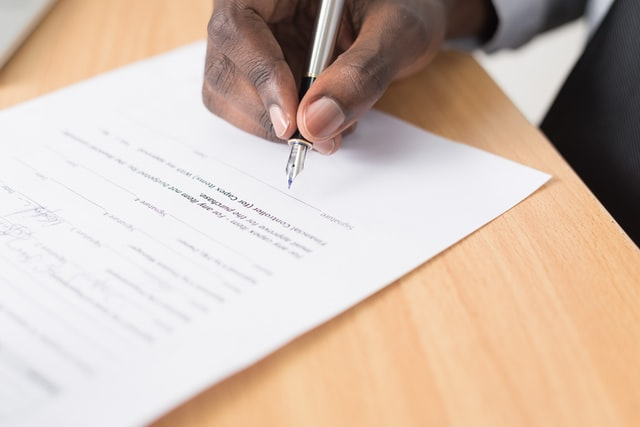
\includegraphics[width=0.75\textwidth]{ContractSigning}
\end{center}
We'll keep using the NBA dataset from the last section; here is the data again for reference:
\begin{center}
{\footnotesize
\begin{tabular}{l l c c l c c c r}
\textbf{Name} & \textbf{Team} & \textbf{No.} & \textbf{Age} & \textbf{Position} & \textbf{Height} & \textbf{Pts} & \textbf{Reb} & \textbf{Salary}\\
\hline
& & & & & & & \\
Jayson Tatum & Celtics & 0 & 22 & PF & 2.03 m & 23.4 & 7.0 & \$7,830,000\\
Joe Harris & Nets & 12 & 28 & SF & 1.98 m & 14.5 & 4.3 & \$7,666,667\\
RJ Barrett & Knicks & 9 & 20 & SG & 1.98 m & 14.3 & 5.0 & \$7,839,960\\
Ben Simmons & 76ers & 25 & 24 & PG & 2.08 m & 16.4 & 7.8 & \$8,113,930\\
Matt Thomas & Raptors & 21 & 26 & SG & 1.93 m & 4.9 & 1.5 & \$898,310\\
Daniel Gafford & Bulls & 12 & 21 & PF & 2.08 m & 5.1 & 2.5 & \$898,310\\
Andre Drummond & Cavaliers & 3 & 27 & C & 2.08 m & 17.7 & 15.2 & \$27,093,019\\
Langston Galloway & Pistons & 9 & 28 & SG & 1.85 m & 10.3 & 2.3 & \$7,333,333\\
Justin Holiday & Pacers & 8 & 31 & SF & 1.98 m & 8.3 & 3.3 & \$4,767,000\\
Khris Middleton & Bucks & 22 & 29 & SF & 2.01 m & 20.9 & 6.2 & \$30,603,448\\
Skal Labissiere & Hawks & 7 & 24 & PF & 2.08 m & 5.8 & 5.1 & \$2,338,847\\
PJ Washington & Hornets & 25 & 22 & PF & 2.01 m & 12.2 & 5.4 & \$3,831,840\\
KZ Okpala & Heat & 4 & 21 & SF & 2.03 m & 1.4 & 1.0 & \$898,310\\
Wes Iwundu & Magic & 25 & 25 & SF & 1.98 m & 5.8 & 2.5 & \$1,618,420\\
Rui Hachimura & Wizards & 8 & 22 & PF & 2.03 m & 13.5 & 6.1 & \$4,469,160\\
Andrew Wiggins & Warriors & 22 & 25 & SF & 2.01 m & 21.8 & 5.1 & \$27,504,630\\
Paul George & Clippers & 13 & 30 & SG & 2.03 m & 21.5 & 5.7 & \$30,560,700\\
Avery Bradley & Lakers & 11 & 29 & PG & 1.91 m & 8.6 & 2.3 & \$4,767,000\\
Jalen Lecque & Suns & 0 & 20 & PG & 1.93 m & 2.0 & 0.4 & \$898,310\\
Harry Giles III & Kings & 20 & 22 & C & 2.11 m & 6.9 & 4.1 & \$2,578,800\\
J.J. Barea & Mavericks & 5 & 36 & PG & 1.78 m & 7.7 & 1.8 & \$1,620,564\\
Bruno Caboclo & Rockets & 5 & 24 & SF & 2.06 m & 3.0 & 2.0 & \$1,845,301\\
Josh Jackson & Grizzlies & 20 & 23 & SG & 2.03 m & 9.0 & 3.1 & \$7,059,480\\
JJ Redick & Pelicans & 4 & 36 & SG & 1.91 m & 15.3 & 2.5 & \$13,486,300\\
Trey Lyles & Spurs & 41 & 24 & C & 2.06 m & 6.4 & 5.7 & \$5,500,000\\
Troy Daniels & Nuggets & 30 & 29 & SG & 1.93 m & 4.3 & 1.1 & \$384,541\\
Naz Reid & Timberwolves & 11 & 21 & C & 2.06 m & 9.0 & 4.1 & \$898,310\\
Luguentz Dort & Thunder & 5 & 21 & SG & 1.91 m & 6.8 & 2.3 & \$155,647\\
Jusuf Nurkic & Trail Blazers & 27 & 26 & C & 2.13 m & 17.6 & 10.3 & \$13,125,000\\
Donovan Mitchell & Jazz & 45 & 23 & SG & 1.85 m & 24.0 & 4.4 & \$3,625,760
\end{tabular}}
\end{center}

Now, let's say a young player is getting ready to sign his first contract.  Before he does, though, he wants to get a sense of what he can expect to earn, and he decides to use this sample of current players to do so.  How would he go about doing this?\\

\subsection{Measures of Center and Spread}
In the last section, we saw how to visualize a full dataset and gain a snapshot understanding of it.  Visuals are good, and they are generally used at the beginning of a study to get a thousand-foot view.  However, if we want to dig deeper, we need to turn from visual summaries to numerical summaries, and that's what we'll discuss in this section.

In fact, when we use the word ``statistic,'' we're generally referring to one of these numbers that describe a dataset, like the average, for instance (the first one we'll cover).  The statistics we'll use in this section can be broadly divided into two categories: \textbf{measures of center} and \textbf{measures of spread}.

\begin{proc}{Center and Spread}
\textbf{Measures of Center:} these give us a sense of what a typical value in the dataset looks like.\\

\textbf{Measures of Spread:} these describe how much variety the dataset contains.\\

\textit{These terms on their own are not important to memorize; they simply help us categorize statistics so that we can compare the statistics in one category to each other.}
\end{proc}

For instance, in the example of the young player entering the league and evaluating player salaries, he may want to start by finding out what a typical salary is (and maybe digging deeper to find a typical \emph{rookie} salary); for this, he would use measures of center.  But then he may wonder how close most players are to this typical value--are salaries very spread out, so that he could be far above or below the center, or are they tightly clustered together, so that he can expect to make about the same as the typical player?  For this, he would use measures of spread.\\

Here are the statistics we'll use:
\begin{itemize}
\item Measures of Center:
\begin{enumerate}
\item Average or Mean
\item Median
\item Weighted Mean
\item Mode
\end{enumerate}
\item Measures of Spread:
\begin{enumerate}
\item Range
\item Standard Deviation
\end{enumerate}
\end{itemize}
We will also combine several of these into what is called the \emph{Five Number Summary} and draw a plot called a \emph{boxplot} to illustrate it.

\paragraph{Note on Population and Sample} Recall from the beginning of the chapter that one of the most fundamental concepts in statistics is the use of a sample to estimate the truth about a population (like we're doing by using this sample of NBA players to describe all players in the league).  Thus, we can talk about, for instance, the \emph{sample average} and the \emph{population average}.  For most of the statistics in this section, there will be no difference in how these are calculated, but there is a slight difference in the \emph{standard deviation}.  For the sake of simplicity, we will simply use the sample version (the difference is very small).

\paragraph{Note on Calculations} For each of these statistics, we'll show the formula and calculate a few examples manually.  However, a graphing calculator has the formulas built in, so after calculating a few the long way, we'll show how to get the answers more quickly using the calculator.

\subsection{Average or Mean}
The mean or average is probably the most familiar of these statistics; it is common measure used to get a sense of the center of a dataset.

To calculate the mean, add up all the values in the set and divide by the number of values.  To write this as a formula, we'll use a new notation:
\[\sum x\]
The symbol $\sum$ is the Greek letter \emph{sigma}, and it means to add up whatever follows, so $\sum x$ means ``the sum of $x$,'' so we'll use that to mean ``sum all the values in the dataset.''

\begin{formula}{Mean}
The mean of a sample of size $n$ is \[\overline{x} = \dfrac{\sum x}{n}\]
\end{formula}

The notation for the mean, $\overline{x}$, is read as ``$x$ bar.''  This stands for the mean of a \emph{sample}; the mean of a \emph{population} is written with the Greek letter \emph{mu}, $\mu$, but we won't worry about that.  We'll assume all the datasets in this section are samples.

\begin{example}{Average NBA Salary}
Find the average salary of the players listed in the NBA dataset.

\sol
To calculate the average, simply add the 30 salaries together, then divide the result by 30:
\begin{align*}
\overline{x} &= \dfrac{7,830,000 + 7,666,667 + 7,839,960 + \cdots + 13,125,000 + 3,625,760}{30}\\
&= \dfrac{230,210,897}{30}\\
&= 7,673,697
\end{align*}

The average salary of this sample of players is $\boxed{\$7,673,697}$.
\end{example}

According to Basketball Reference, the average salary for all NBA players for the same season is \$7.7 million.  Notice how the sample average is almost the same; this is the advantage of taking a sample.  We were able to calculate the average of a small group of 30 randomly chosen players, and although the sample average is not \emph{exactly} the same as the population average, it is an excellent estimate for the population value.

\begin{try}
AIDS data indicating the number of months a patient with AIDS lives after taking a new antibody drug are as follows (smallest to largest):
\begin{center}
\begin{tabular}{c c c c c c c c c c}
3 & 4 & 8 & 8 & 10 & 11 & 12 & 13 & 14 & 15\\
15 & 16 & 16 & 17 & 17 & 18 & 21 & 22 & 22 & 24\\
24 & 25 & 26 & 26 & 27 & 27 & 29 & 29 & 31 & 32\\
33 & 33 & 34 & 34 & 35 & 37 & 40 & 44 & 44 & 47\\
\end{tabular}
\end{center}
Calculate the mean.
\end{try}

\subsection{Median}
We have one measure of center; isn't that enough?  Why do we need another?  Why not just always use the mean?

Look back at the NBA dataset carefully.  We found that the average salary is around \$7.7 million; is this really a typical salary?  In other words, could our young player truly expect to make that much?

If you notice, only 11 players (about a third of the group) make more than \$7 million a year.  The average is often not the best measure of a \emph{typical} value; notice that a few players make over \$20 million, which artificially inflates the average.

Think of it this way; there is a minimum salary possible (\$0, or really whatever the league minimum is defined to be), but there is practically no maximum that someone could be paid.  It turns out that this means that most players are clustered on the lower end (relatively speaking), and a few very highly-paid players increase the average value.

Let's take a simpler example; suppose there are 5 people with the following salaries:
\begin{center}
\begin{tabular}{c c c c c}
\$30,000 & \$45,000 & \$50,000 & \$52,000 & \$1,000,000
\end{tabular}
\end{center}

Calculating the mean for this data set yields \$235,400. Does the mean give a true picture for the center of the data? Can we rightfully say the average person in this data set earns roughly \$235,000? Obviously, the answer is no, since 80\%--or 4/5--of the people in this group earn less than \$53,000. When we have an \textbf{outlier}--a number far removed from the majority of data values--in our data, the mean is \emph{skewed}.
\pagebreak

How else can we measure the center?  Well, we can simply look for the \emph{middle} value, when the data is arranged in order.

\begin{formula}{Median}
The median of a sample, denoted with a capital $M$, is the value in the middle of the list when the data is ordered from smallest to largest (or vice versa).\\

If there are an odd number of values, the median is the middle one.  If there are an even number of values, the median is the average of the two middle ones.
\end{formula}

\begin{example}{Median NBA Salary}
Find the median of the salaries listed in the NBA dataset.

\sol
First, we need to arrange the values in order:
\begin{center}
\begin{tabular}{c c c c c c c c c c}
\$155,647 & 
\$384,541 & 
\$898,310 & 
\$898,310 & 
\$898,310\\
\$898,310 & 
\$898,310 & 
\$1,618,420 & 
\$1,620,564 & 
\$1,845,301\\ 
\$2,338,847 & 
\$2,578,800 & 
\$3,625,760 & 
\$3,831,840 & 
\$4,469,160\\
\$4,767,000 & 
\$4,767,000 & 
\$5,500,000 & 
\$7,059,480 & 
\$7,333,333\\
\$7,666,667 & 
\$7,830,000 & 
\$7,839,960 & 
\$8,113,930 & 
\$13,125,000\\
\$13,486,300 & 
\$27,093,019 & 
\$27,504,630 & 
\$30,560,700 & 
\$30,603,448
\end{tabular}
\end{center}

Since there are an even number of salaries, we need to select the middle two (at the end of the third row and the beginning of the fourth row), and take the average of these two.
\begin{center}
\begin{tabular}{c c c c c c c c c c}
\$155,647 & 
\$384,541 & 
\$898,310 & 
\$898,310 & 
\$898,310\\
\$898,310 & 
\$898,310 & 
\$1,618,420 & 
\$1,620,564 & 
\$1,845,301\\ 
\$2,338,847 & 
\$2,578,800 & 
\$3,625,760 & 
\$3,831,840 & 
{\Large\bfseries\color{red} \$4,469,160}\\
{\Large\bfseries\color{red} \$4,767,000} & 
\$4,767,000 & 
\$5,500,000 & 
\$7,059,480 & 
\$7,333,333\\
\$7,666,667 & 
\$7,830,000 & 
\$7,839,960 & 
\$8,113,930 & 
\$13,125,000\\
\$13,486,300 & 
\$27,093,019 & 
\$27,504,630 & 
\$30,560,700 & 
\$30,603,448
\end{tabular}
\end{center}

Find the average of \$4,469,160 and \$4,767,000:
\begin{align*}
M &= \dfrac{\$4,469,160 + \$4,767,000}{2}\\
&= \boxed{\$4,618,080}
\end{align*}
\end{example}

Notice that this is a more typical salary within the group; exactly half of the players make more and half make less.

\begin{try}
Find the median of the following data, representing the number of months an AIDS patient lives after taking a drug:
\begin{center}
\begin{tabular}{c c c c c c c c c c}
3 & 4 & 8 & 8 & 10 & 11 & 12 & 13 & 14 & 15\\
15 & 16 & 16 & 17 & 17 & 18 & 21 & 22 & 22 & 24\\
24 & 25 & 26 & 26 & 27 & 27 & 29 & 29 & 31 & 32\\
33 & 33 & 34 & 34 & 35 & 37 & 40 & 44 & 44 & 47\\
\end{tabular}
\end{center}
\end{try}

Finding the median manually means having to sort the data, which can be tedious.  However, once we have it sorted, we simply have to find the center.  Often this is easy to do manually, especially when the data is organized in rows, but there's another way to find the center of a list of $n$ values; the center position, since it is midway between 1 and $n$, turns out to be the average of 1 and $n$.
\vfill
\pagebreak

\begin{proc}{Where's the Median}
To find the median, we want to be able to quickly figure out what position to count to in the ordered data set.  To do this, calculate \[\dfrac{n+1}{2}\] where $n$ is the size of the data set.
\end{proc}

\begin{itemize}
\item If $n$ is odd, $\dfrac{n+1}{2}$ is a whole number.  Count to that position and there you'll find the median.
\item If $n$ is even, $\dfrac{n+1}{2}$ is halfway between two whole numbers.  Find the average of the values at those two positions.
\end{itemize}

\paragraph{Outliers:} Let's revisit our small income data set:
\begin{center}
\begin{tabular}{c c c c c}
\$30,000 & \$45,000 & \$50,000 & \$52,000 & \$1,000,000
\end{tabular}
\end{center}

The median is \$50,000, which is a more accurate measure of center than the mean, which is \$235,400. This illustrates how the mean is \textit{sensitive} to outliers, whereas the median is \textit{resistant} to outliers. 

\begin{proc}{Mean and Median}
When outliers are present, the median is a better measure of center. When outliers are absent, the mean can be used.
\end{proc}

When trying to decide whether to use the mean or the median as the measure of the center of a data set, compare them to decide if they are drastically different.  Of course, the best policy is to report both of them and compare them to determine whether the data set is symmetric or \textit{skewed}.

\subsection{Calculating Mean and Median from a Frequency Table}
What if we're given a frequency table instead of raw data?  For instance, suppose we want to calculate the average age of the players in our dataset, and we're given the frequency distribution (which we built in the last section):
\begin{center}
\begin{tabular}{c c}
\textbf{Age} & \textbf{Frequency}\\
\hline
& \\
20 & 2\\
21 & 4\\
22 & 4\\
23 & 2\\
24 & 4\\
25 & 2\\
26 & 2\\
27 & 1\\
28 & 2\\
29 & 3\\
30 & 1\\
31 & 1\\
36 & 2
\end{tabular}
\end{center}
(\emph{Notice that in this case, we removed the rows with frequencies of 0, since our focus at the moment is not on visualizing the data spread.})\\

We can, of course, simply reconstruct the dataset from the frequency table by listing two 20's, four 21's, and so on:
\[20, 20, 21, 21, 21, 21, 22, \ldots\]
At that point, we could calculate the mean and median as before.
\pagebreak

However, if we have the frequency table, we can use a shortcut to calculate each answer.

\subsubsection{Mean}
For the mean, notice that if we want to add up all the values
\[20 + 20 + 21 + 21 + 21 + 21 + 22 + \cdots\]
that's the same as multiplying 20 by 2, multiplying 21 by 4, and so on, and adding all these results.

Thus, we can simply multiply each value by its frequency and add these answers; that will give us the total sum more quickly then adding them one at a time.  At that point, we can divide by the size of the dataset (30) to get the average.
\begin{align*}
\overline{x} &= \dfrac{20(2) + 21(4) + 22(4) + 23(2) + \cdots + 31(1) + 36(2)}{30}\\
&= 25.3
\end{align*}

\subsubsection{Median}
To find the center of the dataset, remember that its location can be found using
\[\dfrac{n+1}{2}.\]
Since we have 30 values, the center will be at 
\[\dfrac{30+1}{2} = 15.5.\]
Since this is not a whole number, it means that the center will be between the 15th and 16th values.

Notice that the frequency table has the ages listed in order, and the frequencies help us count through the set.  Simply add up the frequencies as you go: the first two positions hold 20's, the next four positions hold 21's, and so on, so we simply need to add up frequencies until we get to 15 and 16:
\begin{center}
\begin{tabular}{c c l}
\textbf{Age} & \textbf{Frequency} & \\
\hline
& & \\
20 & 2 & {\color{red} 2}\\
21 & 4 & {\color{red} $2+4=6$}\\
22 & 4 & {\color{red} $6+4=10$}\\
23 & 2 & {\color{red} $10+2=12$}\\
24 & 4 & {\color{red} $12+4=$}{\LARGE\bfseries\color{red}16}\\
25 & 2 & \\
26 & 2 & \\
27 & 1 & \\
28 & 2 & \\
29 & 3 & \\
30 & 1 & \\
31 & 1 & \\
36 & 2
\end{tabular}
\end{center}

Notice that both the 15th and 16th positions contain the value 24, so the median will be 24.

\paragraph{Note:} this process for finding the mean and median from a frequency table doesn't work with a \emph{grouped} frequency table, although a similar process can be used to \emph{estimate} the mean and median in that case.
\vfill
\pagebreak

\subsection{Weighted Mean}
So far, in calculating the mean, we've assumed that all the values are equally significant.  However, there are cases in which we are given \emph{weights} for each value.

The most familiar example is probably that of calculating grades.  For instance, suppose that a syllabus lists the following weights:
\begin{center}
\begin{tabular}{l l}
\textbf{Assignment} & \textbf{Weight}\\
\hline
& \\
Test 1 & 20\%\\
Test 2 & 20\%\\
Test 3 & 20\%\\
Homework & 15\%\\
Project & 10\%\\
Final Exam & 15\%
\end{tabular}
\end{center}

Instead of listing percentages, of course, these assignments could also be given using a points system.  The simplest way to do this would be to simply define a total of 100 points; in that case, the 20\% allocated to each test would correspond to 20 points, and so on.  To make grading easier, many people would instead use 1000 points, as shown:
\begin{center}
\begin{tabular}{l l}
\textbf{Assignment} & \textbf{Points}\\
\hline
& \\
Test 1 & 200\\
Test 2 & 200\\
Test 3 & 200\\
Homework & 150\\
Project & 100\\
Final Exam & 150
\end{tabular}
\end{center}

In either case, once each assignment is graded, we can fill in a table like this:
\begin{center}
\begin{tabular}{l l l}
\textbf{Assignment} & \textbf{Score} & \textbf{Points}\\
\hline
& \\
Test 1 & 85\% & 200\\
Test 2 & 92\% & 200\\
Test 3 & 87\% & 200\\
Homework & 95\% & 150\\
Project & 92\% & 100\\
Final Exam & 91\% & 150
\end{tabular}
\end{center}

Notice how this looks more or less like a frequency table; the score on Test 1 accounts for 200 of the points available, so that test earned $(0.85)(200) = 170$ points.  If we continue down the list, the final score is found by multiplying each percentage earned by the total number of points available, then dividing the final answer by 1000.

\begin{example}{Weighted Average}
Find the final score of the student whose grades are listed below, using both the points system and the percentage system for defining weights.
\begin{center}
\begin{tabular}{l l l l}
\textbf{Assignment} & \textbf{Score} & \textbf{Weight} & \textbf{Points}\\
\hline
& \\
Test 1 & 85\% & 20\% & 200\\
Test 2 & 92\% & 20\% & 200\\
Test 3 & 87\% & 20\% & 200\\
Homework & 95\% & 15\% & 150\\
Project & 92\% & 10\% & 100\\
Final Exam & 91\% & 15\% & 150
\end{tabular}
\end{center}

\sol
Using the points given, we can multiply each score by the available points and add these up:
\begin{align*}
\textrm{Points earned } &= (0.85)(200) + (0.92)(200) + (0.87)(200) + (0.95)(150)\\
&\ \ + (0.92)(100) + (0.91)(150)\\
&= 899
\end{align*}
The student's final score, then, is the percentage of available points that they earned:
\[\textrm{Final Grade } = \dfrac{899}{1000} = 0.899 = \boxed{89.9\%}\]

Now, let's do the same thing using the percentage weights instead of possible points.  Here, notice that the percentages are simply the number of points for each category divided by 1000.  In other words, the last step of the calculation (dividing by 1000) is already done for us, so we simply need to multiply the percentage earned by the percentage weight:
\begin{align*}
\textrm{Final Grade } &= (0.85)(0.2) + (0.92)(0.2) + (0.87)(0.2) + (0.95)(0.15)\\
&\ \ + (0.92)(0.1) + (0.91)(0.15)\\
&= 0.899\\
&= \boxed{89.9\%}
\end{align*}
\end{example}

\subsection{Mode}
There is another, less used, measure of center: the mode. 

\begin{formula}{Mode}
The mode is the most frequently occurring value in a dataset.
\end{formula}

There can be more than one mode in a data set as long as those values have the same frequency and the frequency is the highest. A data set with two modes is called \textbf{bimodal}.

\begin{example}{Mode}
Find the mode of the dataset summarized below, the ages of players in the NBA dataset.
\begin{center}
\begin{tabular}{c c}
\textbf{Age} & \textbf{Frequency}\\
\hline
& \\
20 & 2\\
21 & 4\\
22 & 4\\
23 & 2\\
24 & 4\\
25 & 2\\
26 & 2\\
27 & 1\\
28 & 2\\
29 & 3\\
30 & 1\\
31 & 1\\
36 & 2
\end{tabular}
\end{center}

\sol
Since the data is already summarized with a frequency table, all we have to do is scan through and find the highest frequency (4) and check the ages that appear with that frequency.  Thus, the modes (this dataset has three) are \[\boxed{21, 22, 24}\]
\end{example}

\begin{try}
The number of books checked out from the library from 25 students are as follows: 
\begin{center}
\begin{tabular}{c c c c c c c c c c c c c}
0 & 0 & 0 & 1 & 2 & 3 & 3 & 4 & 4 & 5 & 5 & 7 & 7\\
7 & 7 & 8 & 8 & 8 & 8 & 9 & 10 & 10 & 11 & 11 & 12 & 
\end{tabular}
\end{center}
Find the mode.
\end{try}

The mode is not nearly as useful as the other two measures of center (mean and median), so we won't spend as much time on it as on the others.

Now we're ready to turn from measures of center to measures of spread, which we'll use to observe how much variety a dataset contains.
\pagebreak

\subsection{Range}
The \textbf{range} is the simplest measure of spread.  It is simply the distance between the smallest and largest data value in the set, which can be calculated by subtracting them.

\begin{formula}{Range}
The range is the calculated by finding the difference between the minimum and maximum value in a dataset:
\[\textrm{Range } = \textrm{ Maximum } - \textrm{ Minimum}\]
\end{formula}

\begin{example}{Range of NBA Players' Heights}
Find the range of heights for the NBA players listed in the dataset at the beginning of the chapter.

\sol
All we have to select from the list is the smallest value and the largest value.  Scanning the list reveals that the minimum is 1.78 meters and the maximum is 2.13 meters.  The range, then, is simply the difference between these two:
\begin{align*}
\textrm{Range } &= 2.13 - 1.78\\
&= \boxed{0.35 \textrm{ m}}
\end{align*}
\end{example}

This relatively small range means that there is not much variation in the heights of the players in our sample.\\

How do we distinguish a small range from a large one?  The key is to compare the range to a typical value.  For instance (and this isn't the only way to do this), if we calculate the range as a percentage of the mean (the mean height is 1.99 m), we get
\[\dfrac{0.35}{1.99} = 18\%\]

On the other hand, the range of the points scored is much larger compared to its mean.  The range of that list is 22.6, while the mean is 11.28, so the range is approximately 200\% as large as the mean.  By comparison, there is clearly much more variation within the points column than the players' heights.

\subsection{Standard Deviation}

The \textbf{standard deviation} is a number that measures how far a typical data value is from the mean. The standard deviation is always positive or zero. A small standard deviation means less spread in the data; a large standard deviation means more spread in the data.\\

First of all, the \textbf{deviation} of each data point $x$ is its difference from the mean $\overline{x}$:
\[x-\overline{x}.\]
Each value in the data set has a deviation associated with it.  If we want to find how far, on average, each data point is from the mean, it would make sense to take the average of the deviations.  However, there's a problem with doing that: if we add up the deviations, we'll always get 0, because of the way that $\overline{x}$ is calculated.  Some of the deviations are positive, some are negative, and the positives cancel out the negatives.

\marginnote{It is not quite an average, since we divide by $n-1$ instead of $n$.  The reasons for this are complicated, but they have to do with making the sample variance be what is called an unbiased estimator for the population variance.}
To get around this, we square the deviations so that everything becomes positive.  NOW, when we take an average\footnote{\textit{almost; see margin note}} of these \textit{squared} deviations, we get a meaningful number, instead of getting 0 every time.  We call this ``average'' the variance:
\[s^2 = \dfrac{\sum (x-\overline{x})^2}{n-1}\]

The only problem now is that we've got an average of these squared things, so the units of our answer are not the same units we started with.  In other words, if the data is given in units of inches, we've got a variance in square inches.  To get an answer, we take the square root of the variance, and that's what we call the standard deviation.
\[\textrm{s} = \sqrt{\frac{\Sigma (x - \overline{x})^2}{n-1}}\]

To calculate the standard deviation,
\begin{enumerate}
\item Calculate the mean of the data values, $\overline{x}$.
\item Subtract the mean from each data value to find the deviations: 
\[\textrm{deviation } = x - \overline{x}\]
\item Square each deviation: $(x - \overline{x})^2$
\item Take the sum of the squared deviations: $\Sigma (x - \overline{x})^2$
\item Divide that sum by $n$ minus 1, where $n$ is the number of data values: $\frac{\Sigma (x - \overline{x})^2}{n-1}$
\item Take the square root of this quotient: $\sqrt{\frac{\Sigma (x - \overline{x})^2}{n-1}}$
\end{enumerate}

\begin{formula}{Standard Deviation}
The standard deviation of a sample is given by
\[\textrm{s} = \sqrt{\frac{\Sigma (x - \overline{x})^2}{n-1}}\]
where $n$ stands for the number of data values and $x$ stands for each data value.
\end{formula}

Don't worry; we'll use this formula once to calculate the standard deviation, and then let the calculator handle the tedious calculation for us.

\begin{example}[https://www.youtube.com/watch?v=jdDlgDV96JE]{At the Mall}
Kari went shopping and bought five things. The prices are as follows:
\begin{center}
\begin{tabular}{c c c c c}
\$20 & \$4 & \$15 & \$9 & \$3
\end{tabular}
\end{center}
Calculate the standard deviation for this data.

\sol
\[\overline{x} = (20 + 4 + 15 + 9 + 3) / 5 = 10.20\]
The mean is \$10.20. We can use the table below to get the standard deviation.\\

\begin{center}
\begin{tabular}{c | c | c} 
\textbf{Data Value} & \textbf{Deviations} & \textbf{Deviations$^2$}\\
$x$ & $(x - \overline{x})$ & $(x - \overline{x})^2$\\
\hline
20 & $20-10.20=9.8$ & $(9.8)^2=96.04$\\
4 & $4-10.20=-6.2$ & $(-6.2)^2=38.44$\\
15 & $15-10.20=4.8$ & $(4.8)^2=23.04$\\
9 & $9-10.20=-1.2$ & $(-1.2)^2=1.44$\\
3 & $3-10.20=-7.2$ & $(-7.2)^2=51.84$
\end{tabular}
\end{center}
Adding up all the values in the third column yields 210.8. The variance, $s^2$, is equal to this sum divided by the total number of data values minus one.

\[s^2 = \dfrac{210.8}{5-1} = \$52.7. \]
The standard deviaion $s$ is equal to the square root of the variance.
\[s = \sqrt{52.7} = \boxed{\$7.26}\]
\end{example}
\pagebreak

\subsection{Using Your Calculator}
For each of the statistics in this section, we've shown how to calculate them manually.  Just as a reminder, we now know how to calculate each of the following for a dataset:
\begin{itemize}
\item Measures of Center:
\begin{enumerate}
\item Average or Mean
\item Median
\item Weighted Mean
\item Mode
\end{enumerate}
\item Measures of Spread:
\begin{enumerate}
\item Range
\item Standard Deviation
\end{enumerate}
\end{itemize}

Most of these (with the exception of the mode and the range) can be found directly in a list of statistics that a TI calculator calls \texttt{1-Var Stats}.  This list can be generated for a dataset entered in the calculator.  The range can also be calculated indirectly from this list, but we'll have to stick to the manual method for finding the mode (thankfully, this is pretty simple).\\

To begin, enter a dataset as before; press the \calcbutton{STAT} button, then \calcbutton{ENTER} to enter the \texttt{Edit} menu.  We'll use the points per game listed in the NBA dataset to illustrate the process.
\begin{center}
\begin{tabular}{c c c}
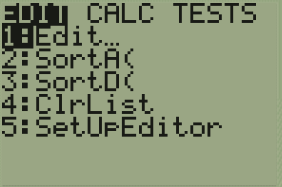
\includegraphics[height=0.8in]{gmRegression1}
& 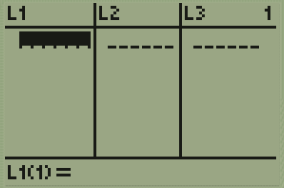
\includegraphics[height=0.8in]{gmRegression2}
& 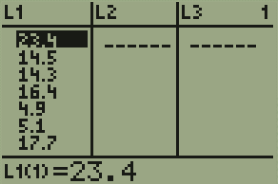
\includegraphics[height=0.8in]{PointsCalculator}
\end{tabular}
\end{center}

Next, press the \calcbutton{STAT} button again, and use the right arrow key to navigate over to the \texttt{CALC} menu.  Select the first option, labeled \texttt{1: 1-Var Stats}.  Since we entered the data in \texttt{L1}, we can leave the default options alone and simply select \texttt{Calculate}.
\begin{center}
\begin{tabular}{c c c}
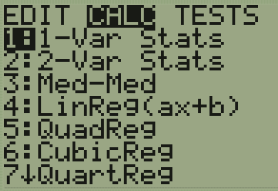
\includegraphics[height=0.8in]{1VarStats1}
& 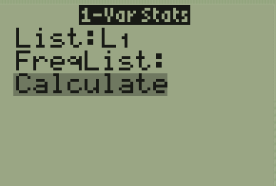
\includegraphics[height=0.8in]{1VarStats2}
& 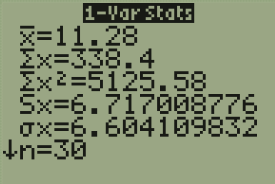
\includegraphics[height=0.8in]{1VarStats3}
\end{tabular}
\end{center}

This list contains many statistics; notice that the first one is labeled $\overline{\texttt{x}}$; this, of course, is the mean.  The next is $\sum\texttt{x}$, or the sum of the values, and the one after that is the sum of the squares (we haven't used either of these values directly).

After that, notice the value of $\texttt{S}_\texttt{x}$; this is the standard deviation for the sample.  The next value is the population standard deviation, which we can ignore (if you take a statistics course, you can worry about the difference then).

Scrolling down using the arrow keys reveals a few more statistics, which we will investigate a bit more fully at the end of this section, when we discuss the Five Number Summary:
\begin{center}
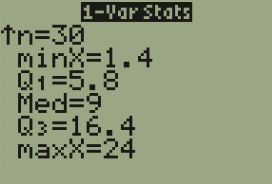
\includegraphics[height=1in]{1VarStats4}
\end{center}
For now, notice that \texttt{minX} and \texttt{maxX}, the minimum and maximum values, can be used to calculate the range.  Also, the median is listed, labeled \texttt{Med}.

\subsubsection{Frequency Tables and Statistics}
Remember how we calculated the mean and median of a dataset using a frequency table earlier (and a weighted mean uses the same process)?  We can also do this using the calculator; let's illustrate using the age data for the NBA players; refer to the earlier discussion of mean and median with a frequency table to see the distribution.
\pagebreak

Now, when we enter the data, we'll enter the ages in \texttt{L1} and the frequencies in \texttt{L2}, and this time, in the \texttt{1-Var Stats} menu, change the \texttt{FreqList} option to \texttt{L2} (press \calcbutton{2ND} \calcbutton{2} to write \texttt{L2}):
\begin{center}
\begin{tabular}{c c c}
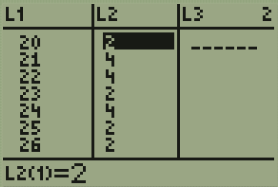
\includegraphics[height=0.8in]{1VarStats5}
& 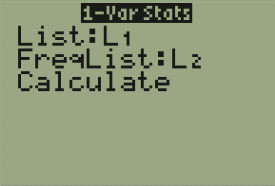
\includegraphics[height=0.8in]{1VarStats6}
& 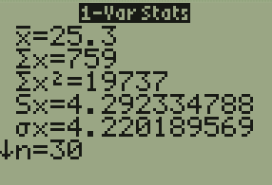
\includegraphics[height=0.8in]{1VarStats7}
\end{tabular}
\end{center}

The mean is 25.3, the same value we calculated manually, and the other values can be found in the list as well.

\subsection{Using Excel}
All of these statistics can be calculated using built-in Excel formulas; for each, enter the formula name, followed by open parentheses, then select the cells you want to use for the calculation, and close the parentheses.

Here are the formulas:
\begin{center}
\begin{tabular}{l l l}
\textbf{Statistic} & \textbf{Formula} & \\
\hline
& & \\
Mean & \texttt{AVERAGE(cells)} & \\
& & \\
Median & \texttt{MEDIAN(cells)} & \\
& & \\
Mode & \texttt{MODE.MULT(cells)} & \parbox{2in}{The \texttt{MULT} part means that this will return multiple values; results will spill over into the cells below the one with the formula.}\\
& & \\
Range & \texttt{MAX(cells) - MIN(cells)} & \parbox{2in}{As with the calculator, the range must be calculated indirectly.}\\
& & \\
Standard Deviation & \texttt{STDEV.S(cells)} & \parbox{2in}{The \texttt{S} refers to the fact that this is the \emph{sample} standard deviation; for the population standard deviation, use \texttt{STDEV.P}.}
\end{tabular}
\end{center}

For example, the following spreadsheet shows the results for all of the numerical variables in the NBA dataset:
\begin{center}
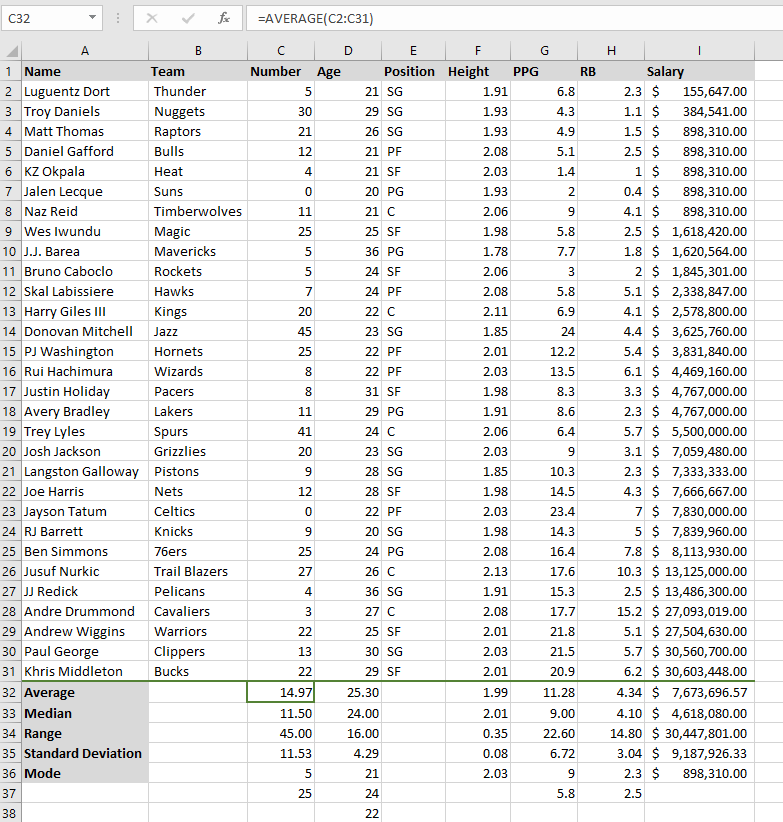
\includegraphics[height=3.75in]{Excel1VarStats}
\end{center}
\pagebreak

\subsection{Five Number Summary and Boxplot}
Let's go back to the bottom of the \texttt{1-Var Stats} results from the calculator:
\begin{center}
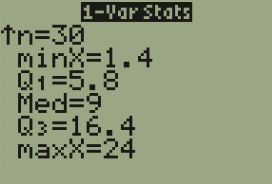
\includegraphics[height=1.5in]{1VarStats4}
\end{center}

We've already discussed the median, and how it splits the data in half.  In other words, half of the players averaged fewer than 9 points per game, and half scored above that.  So between the minimum of 1.4 and the median, you'll find half of the players, and between the median and the maximum of 24, you'll find the other half.\\

What about those other two values ($\texttt{Q}_\texttt{1}$ and $\texttt{Q}_\texttt{3}$)?  These, it turns out, continue the process of division in half.  Specifically, $Q_1$ divides the lower half of players in half again (it is the median of the lower half) and $Q_3$ divides the upper half in half again.\\

Thus, these five numbers (the minimum, $Q_1$, the median, $Q_3$, and the maximum) split the data into quarters, and a quarter of the players fall into each of these divisions.  This is where the $Q$ notation comes from: $Q_1$ is called the \textbf{first quartile} and $Q_3$ is called the \textbf{third quartile}.  The median is sometimes called the \textbf{second quartile}, and it can be denoted by $Q_2$ (instead of the $M$ we used earlier).\\

\begin{formula}{Five Number Summary}
The Five Number Summary lists the following values:
\begin{itemize}
\item Minimum
\item First Quartile
\item Median
\item Third Quartile
\item Maximum
\end{itemize}
These values divide the dataset into four divisions, and a quarter of the data values fall into each division.
\end{formula}

The value in these five values (which together are called the \emph{Five Number Summary}) is that they can give us a sense of where the data is clustered or spread out.\\

For instance, the first quarter of the data in the example above falls between 1.4 and 5.8 (a range of 4.4), the second quarter is between 5.8 and 9 (a range of 3.2), the third between 9 and 16.4 (7.4), and the last between 16.4 and 24 (7.6).\\

Notice how the ranges are tighter on the lower end; this indicates grouping on the low side, since values are packed in more closely.  On the upper end, we have to cover a spread of 7 or 8 points to find the same number of players that 3 or 4 points covered on the lower end.
\vfill
\pagebreak

Since it can be hard to interpret these results when they're given as a list of number like this, we can draw a graph to visualize the Five Number Summary, called a \emph{boxplot}.

\begin{formula}{Boxplot}
A boxplot is a visual representation of a Five Number Summary.  It consists of vertical lines marking each of the five values.  The middle three (from the first quartile to the third quartile) are joined with a box, giving the plot its name.  Lines are drawn from this box out to the minimum and maximum; these lines are called \emph{whiskers}, so that these plots are sometimes called box-and-whisker plots.

\begin{center}
\begin{tikzpicture}
\begin{axis}[
ymax=2,
ymin=0,
xmin=39.9,
xmax=48.1,
y=1.5cm,
xtick={40,41,...,48},
xticklabels={,,,,,,,,},
yticklabels={},
axis y line=none,
axis x line=bottom,
%axis lines=none,
%ytick={1,2,3},
%yticklabels={Group A, Group B, Group C},
]
\addplot+[black,thick,
boxplot prepared={
lower whisker=41, lower quartile=44,
median=45,
upper quartile=46, upper whisker=47,
},
]
coordinates {}
[above]
node at
(boxplot box cs: \boxplotvalue{lower whisker},1)
{Min}
node at
(boxplot box cs: \boxplotvalue{lower whisker},-0.5)
{Lower Whisker}
node at
(boxplot box cs: \boxplotvalue{lower quartile},1)
{$Q_1$}
node at
(boxplot box cs: \boxplotvalue{median},1)
{$Q_2$}
node at
(boxplot box cs: \boxplotvalue{median},-0.5)
{Median}
node at
(boxplot box cs: \boxplotvalue{upper quartile},1)
{$Q_3$}
node at
(boxplot box cs: \boxplotvalue{upper whisker},1)
{Max}
node at
(boxplot box cs: \boxplotvalue{upper whisker},-0.53)
{Upper Whisker}
;

\end{axis}
\end{tikzpicture}
\end{center}
\end{formula}

For instance, the boxplot for the players' scoring would look like the following:
\begin{center}
\begin{tikzpicture}
\begin{axis}[
ymax=2,
y=1.5cm,
xtick={1,2,...,24},
xticklabels={,2,,4,,6,,8,,10,,12,,14,,16,,18,,20,,22,,24},
yticklabels={},
axis y line=none,
axis x line=bottom,
xmin=0,
xmax=25,
%ytick={1,2,3},
%yticklabels={Group A, Group B, Group C},
]
\addplot+[black,thick,
boxplot prepared={
lower whisker=1.4, lower quartile=5.8,
median=9,
upper quartile=16.4, upper whisker=24,
}, /pgf/number format/precision=1
]
coordinates {}
[above]
node at
(boxplot box cs: \boxplotvalue{lower whisker},1)
{\pgfmathprintnumber{\boxplotvalue{lower whisker}}}
node at
(boxplot box cs: \boxplotvalue{lower quartile},1)
{\pgfmathprintnumber{\boxplotvalue{lower quartile}}}
node at
(boxplot box cs: \boxplotvalue{median},1)
{\pgfmathprintnumber{\boxplotvalue{median}}}
node at
(boxplot box cs: \boxplotvalue{upper quartile},1)
{\pgfmathprintnumber{\boxplotvalue{upper quartile}}}
node at
(boxplot box cs: \boxplotvalue{upper whisker},1)
{\pgfmathprintnumber{\boxplotvalue{upper whisker}}}
;

\end{axis}
\end{tikzpicture}
\end{center}

Notice how the lower side is more scrunched together, and the upper side is more spread out; this is the same thing we observed from the values themselves, but it's easier to see on a picture.\\

The graphing calculator can also draw these; if you open the \texttt{STAT PLOT} menu and select one of the plots, you can see the option for a boxplot.  Notice that there are two types; one separates \emph{outliers} from the data, which we haven't discussed here, so we'll use the second version (without the dots).  After adjusting the window, we can view the plot (note that to see the values of the bars, we can use the \calcbutton{TRACE} button).
\begin{center}
\begin{tabular}{c c c}
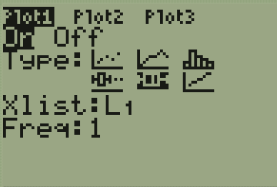
\includegraphics[height=0.9in]{CalculatorBoxplot}
& 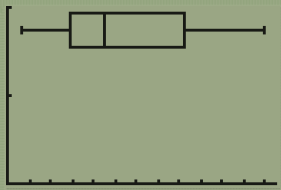
\includegraphics[height=0.9in]{CalculatorBoxplot2}
& 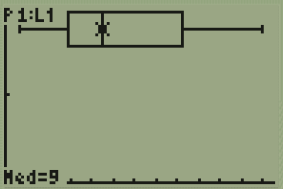
\includegraphics[height=0.9in]{CalculatorBoxplot3}
\end{tabular}
\end{center}